% \section{分层仿真平台}
ROS利用URDF(\underline{U}nified \underline{R}obot \underline{D}escription \underline{F}ormat)描述机器人模型,URDF通过xml格式对机器人系统的模型、驱动器、传感器和场景等进行组织,开发者只需添加相应的标签对上述属性进行定义。同时,该文件提供了一套便于控制程序与Gazebo进行信息交流的机制。为提高系统的鲁棒性、可扩展性,本文根据ROS松耦合的特性,建立了基于关节控制、动作执行和行为生成三层系统架构的仿真平台。

\section{关节控制层}
% 操作臂是由一系列刚体通过关节连接而成的运动链\cite{johnj.craigJiQiRenXueDaoLun2006}。一个基本的机器人系统应当包含对其全部连杆的位姿、质量和惯性矩阵的定义以及相应关节的位置、类型等的描述。此外,在仿真环境中一般还需对机器人的视觉属性和碰撞属性进行定义,前者便于用户查看仿真环境中机器人的状态,后者为ROS进行碰撞计算提供依据。一个基础的机器人模型定义如下。

% \lstset{
%     columns=fixed,
%     numbers=left,                                        % 在左侧显示行号
%     frame=none,                                          % 不显示背景边框
%     backgroundcolor=\color[RGB]{245,245,244},            % 设定背景颜色
%     keywordstyle=\color[RGB]{40,40,255},                 % 设定关键字颜色
%     numberstyle=\footnotesize\color{darkgray},           % 设定行号格式
%     commentstyle=\it\color[RGB]{0,96,96},                % 设置代码注释的格式
%     stringstyle=\rmfamily\slshape\color[RGB]{128,0,0},   % 设置字符串格式
%     showstringspaces=false,                              % 不显示字符串中的空格
%     language=xml,                                        % 设置语言
%     morekeywords={name, type},
%     emph={robot, link, joint},
%     emphstyle=\color{CodeViolet}
% }
% {\renewcommand\baselinestretch{1.0}\selectfont
% {\setmainfont{Courier New Bold}                          % 设置代码字体
% \begin{lstlisting}
% <robot name="robot">
%     <link name="link1" />
%     <link name="link2" />

%     <joint name="joint" type="continuous">
%         <parent link="link1" />
%         <child link="link2" />
%     </joint>
% </robot>
% \end{lstlisting}}
% \par}

% ROS提供了部分简单的模型便于用户对视觉属性及碰撞属性进行定义,这些模型包括圆柱体(Cylinder)、球体(Sphere)等,但这些模型难以对复杂的形状进行描述。ROS提供的sw\_urdf\_exporter插件有助于解决这一问题,开发者只需在计算机辅助建模软件中建立相应的机械模型,定义相关的连杆质量、惯性矩阵和关节的种类、位置及运动范围等信息,即可生成urdf文件,大大简化了机器人系统的构建过程。由此建立的仿生机器鼠模型如图\ref{figure_rosmodel}。
% \begin{figure}[htbp]
%   %\vspace{13pt}
%   \centering
%   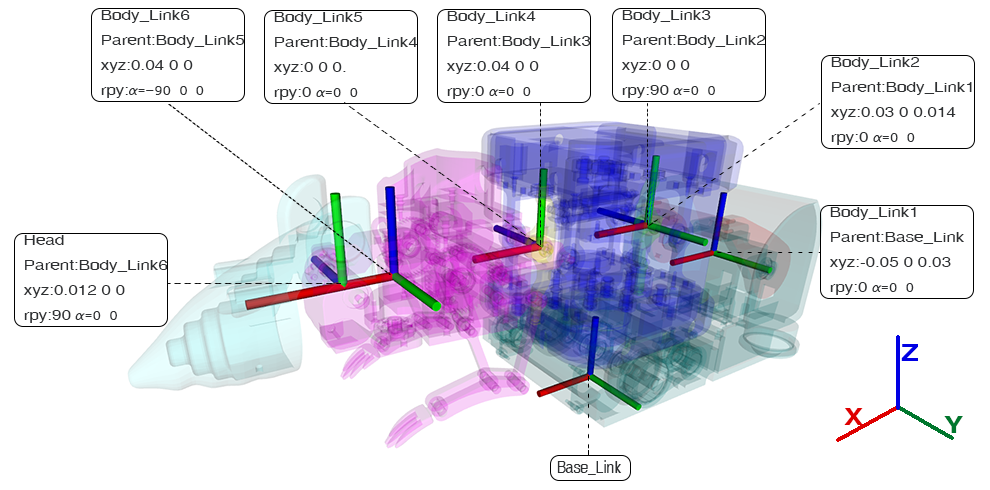
\includegraphics[width=0.95\linewidth]{images/ch03/frame.png}
%   \caption{仿生机器鼠模型及其关节位置}\label{figure_rosmodel}
% \end{figure}

% ros\_control包提供了控制Gazebo仿真环境和真实世界中机器人关节的硬件接口、控制器接口、传动装置接口、控制器工具箱等,本文使用其控制Gazebo中的机器鼠,为此需要在参数文件yaml中定义各关节控制器及其类型,并将其加载至Controller Manager中进行管理。这些控制器包括:控制驱动轮的关节速度控制器、控制躯干各关节的关节轨迹控制器及获取、发布关节信息的关节状态控制器。

% 同时,为使Gazebo能够正确导入相应的关节和控制器信息,需要在URDF文件中添加相关声明。

% 配置完成后的系统信息流如图\ref{figure_bottomlayer}。其中,Controller Manager中的Joint State Controller负责获取仿生机器鼠各关节的状态信息(包括位置、速度和加速度)并进行发布,其数据同时作为关节控制器的反馈量。其余Controller由上层控制器进行控制,并转化为相应的关节速度或位置输出。Hardware Resource Interface将Controller Manager和Simulation隔离,提高平台的复用性,当系统迁移至实体机器鼠时,不必做额外改动。Simulation通过readSim()直接读取关节状态并向上反馈,通过writeSim()直接控制Gazebo中模型的关节运动。

如图\ref{figure_bottomlayer}所示,关节控制层的主要作用为完成对Gazebo中仿生机器鼠模型各关节控制方式的抽象,并为上层控制器提供相应的程序接口,提高复用率和仿真平台的稳定性。
\begin{figure}[htb]
  %\vspace{13pt}
  \centering
  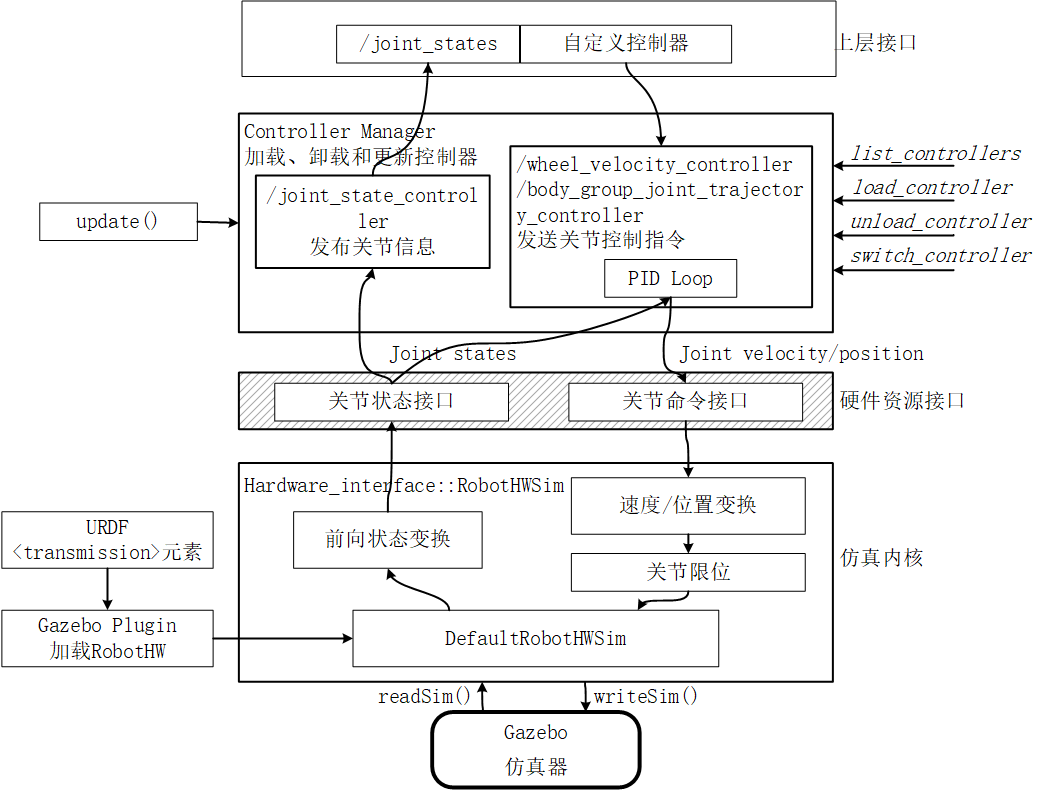
\includegraphics[width=0.55\linewidth]{images/ch03/bottomlayer.png}
  \caption{关节控制层数据流图}\label{figure_bottomlayer}
\end{figure}

%而对机器鼠身体部分的关节而言,其运动指令主要受限于关节位置的合法性,因此只需保证其位置控制指令在合理区间即可,相应各个关节的运动范围如表\ref{table_jointlimit}。

\section{动作执行层}
动作即为一个或数个关节相互配合的运动,在关节控制层已搭建的基础上,仿真系统将依靠调用相关的控制接口实现特定动作。

仿生机器鼠的动作分为两大主要板块:轮部运动和躯干运动。在关节控制层中,机器鼠轮部关节控制器为速度控制器,订阅机器鼠所命名空间下的\//left\_wheel\_joint\_ve-\linebreak[1]locity和\//right\_wheel\_joint\_velocity话题。因此在动作执行层中,只需向上述话题发布速度指令即可完成控制。

% 现有研究表明,生物鼠在剧烈运动和缓和运动时运动速度分别保持在一定范围内\cite{whishawBehaviorLaboratoryRat2005},这为控制机器鼠运动速度提供了参考。为使机器鼠运动速度与生物鼠相适应,其轮部关节运动速度将按照式\ref{equation_velocity}计算。
% \begin{equation}\label{equation_velocity}
%   \left[\begin{array}{c}
%           \omega_{r} \\
%           \omega_{l}
%         \end{array}\right]=\left[\begin{array}{cc}
%                                    1/2 & l/2r \\
%                                    1/2 & -l/2r
%                                  \end{array}\right]\left[\begin{array}{c}
%                                                             v_{c} \\
%                                                             \omega_{c}
%                                                           \end{array}\right].
% \end{equation}

% 式\ref{equation_velocity}中,$\omega_{l}$和$\omega_{r}$分别表示机器鼠左轮和右轮的角速度,$v_{c}$表示机器鼠线速度,$\omega_{c}$表示其角速度,$l$表示机器鼠轮距($32~mm$),$r$表示轮半径($10~mm$),将$v_{c}=10~cm/s, \omega_{c}=0$代入式中,计算得$\omega_{l}=\omega_{r}=10~rad/s$,表示仿生机器鼠直线前进或后退时,两轮角速度应为$10~rad/s$。
% \begin{figure}[htbp]
%   %\vspace{13pt}
%   \centering
%   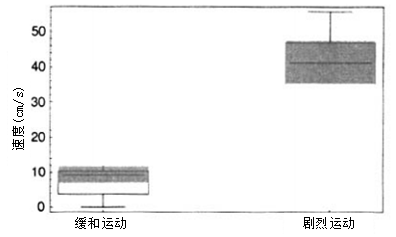
\includegraphics[width=0.6\linewidth]{images/ch03/velocity.png}
%   \caption{生物鼠缓和运动和剧烈运动时速度范围\cite{whishawBehaviorLaboratoryRat2005}}\label{figure_ratspd}
% \end{figure}

% 仿生机器鼠躯干部分运动涉及到机械臂的运动规划,这一部分将依靠MoveIt包实现。

% MoveIt是ROS中集合了与机械臂移动操作相关的组件包的运动规划库。它提供了运动规划中所需要的大部分功能,同时提供友好的配置和调试界面便于完成机器人在ROS系统上的初始化及调试,其系统架构如图\ref{figure_moveit}。
% \begin{figure}[htb]
%   %\vspace{13pt}
%   \centering
%   \includegraphics[width=0.8\linewidth]{images/ch03/moveit_pipeline.png}
%   \caption{MoveIt系统架构}\label{figure_moveit}
% \end{figure}

% 图\ref{figure_moveit}显示,Move\_group是MoveIt的核心节点,它将MoveIt的所有组件(规划场景、规划流程和执行器)集成起来,并提供了一系列动作和服务供用户使用,用户可以用c++、python或者图形界面调用这些动作和服务。

% 图\ref{figure_moveit}中,Move\_group能够根据机器鼠当前所处的场景(Planning Scene)和关节状态(Joint State    ),调用开源运动规划库 (OMPL)或其他运动规划库,完成机器鼠的动作规划,并通过动作JointTrajectoryAction调用机器鼠的控制器。为完成这一过程,需要提供SRDF(\underline{S}emantic \underline{R}obot \underline{D}escription \underline{F}ormat)文件,它是MoveIt针对控制机器人关节运动使用的一种机器人描述文件格式。它基于URDF对机器人的描述,对关节组、默认状态、附加碰撞检测信息和附加坐标系变换进行定义,利用moveit\_setup\_assistant可以基于完整的URDF文件生成SRDF文件,其过程为:

% \begin{enumerate}[leftmargin=0em, listparindent=2em, parsep=0em, topsep=0em, label=(\theenumi)]
% %\setlength{\leftmargin}{0em}
% \setlength{\itemindent}{4em}
% \setlength{\labelsep}{0em}
% \setlength{\labelwidth}{2em}
% \setlength{\parsep}{0em}
% \setlength{\itemsep}{0em}
% \setlength{\topsep}{0em}
% %\setlength{\listparindent}{2em}
%   \item 导入URDF文件。
%   \item 生成自碰撞矩阵。自碰撞矩阵记录各连杆之间的碰撞可能性,使某些情况下啊可以安全地关闭碰撞检测,减少运动规划处理地时间。这一过程涉及地参数为采样比重,本文采取其默认值$10000$。
%   \item 添加虚拟关节。虚拟关节定义机器人或机械臂与世界坐标系的连接方式,本文仿生机器鼠为移动机器人,不需添加虚拟关节。
%   \item 添加规划组。规划组是对机器人机构中某一部分的描述,包含其中一些连杆和关节。本文将机器鼠躯干部分定义为一个规划组rat\_body\_group,将base\_link作为其正运动学的起始连杆,将head作为其末端连杆,选择KDL作为其正运动学求解器。
%   \item 添加机器人位姿。将表\ref{table_jointpos}中规划的机器鼠动作对应的各关节位置作为仿生机器鼠的位姿,其结果如图\ref{figure_ratbot_pose}。
% \begin{figure}[htbp]
%   %\vspace{13pt}
%   \centering
%   \subfigure[直立]{\label{figure_ratbot_pose_rear}
%   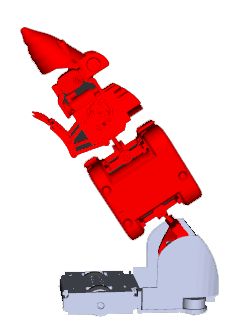
\includegraphics[width=0.10\linewidth]{images/ch03/pose/03rear.png}
%   }
%   \subfigure[嗅探]{\label{figure_ratbot_pose_sniff}
%   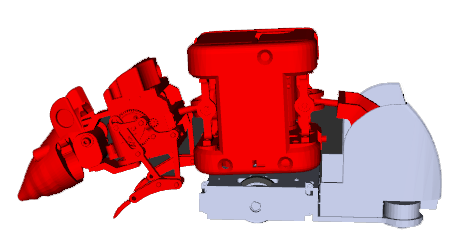
\includegraphics[width=0.15\linewidth]{images/ch03/pose/04sniff.png}
%   }
%   \subfigure[梳理]{\label{figure_ratbot_pose_groom}
%   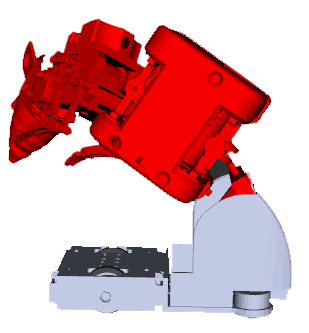
\includegraphics[width=0.13\linewidth]{images/ch03/pose/05groom.png}
%   }
%   \subfigure[被梳理]{\label{figure_ratbot_pose_subgroom}
%   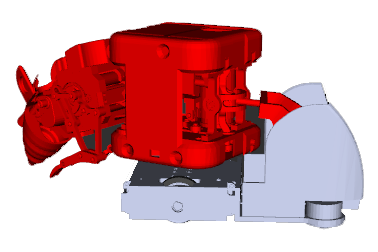
\includegraphics[width=0.15\linewidth]{images/ch03/pose/06subgroom.png}
%   }
%   \subfigure[攀爬]{\label{figure_ratbot_pose_up}
%   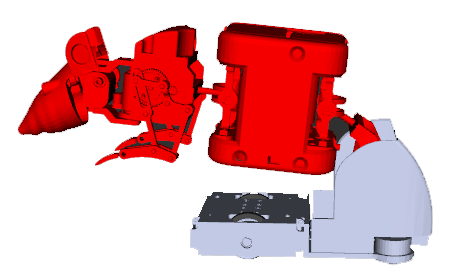
\includegraphics[width=0.15\linewidth]{images/ch03/pose/07up.png}
%   }
%   \subfigure[匍匐]{\label{figure_ratbot_pose_under}
%   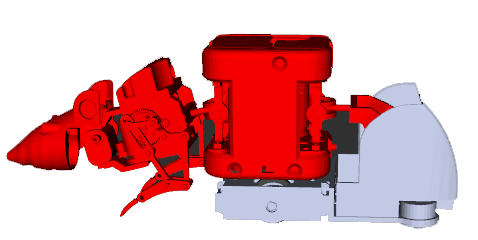
\includegraphics[width=0.15\linewidth]{images/ch03/pose/08under.png}
%   }
%   \caption{利用moveit\_setup\_assistant实现机器鼠位姿}\label{figure_ratbot_pose}
% \end{figure}
%   \item 标记末端执行器。对执行抓取、切割等操作的机械臂而言,标记末端执行器能够更好地执行相应操作,但本文中仿生机器鼠无此类要求,因此未标记末端执行器。
%   \item 添加被动关节。本文所使用的机器鼠所有关节均为主动关节,因此不需添加被动关节。
%   \item 生成配置文件。
% \end{enumerate}

% 完成上述过程后,用户能够通过MoveIt提供的c++、python接口或图形化控制界面完成机器鼠预定义位姿、笛卡尔空间和关节空间的动作控制。一个典型的的动作执行过程包含规划(plan)和执行(execute)两部分,利用c++接口实现机器鼠运动至直立位姿的代码如下。

% \lstset{
%     columns=fixed,
%     numbers=left,                                        % 在左侧显示行号
%     frame=none,                                          % 不显示背景边框
%     backgroundcolor=\color[RGB]{245,245,244},            % 设定背景颜色
%     keywordstyle=\color[RGB]{40,40,255},                 % 设定关键字颜色
%     numberstyle=\footnotesize\color{darkgray},           % 设定行号格式
%     commentstyle=\it\color[RGB]{0,96,96},                % 设置代码注释的格式
%     stringstyle=\rmfamily\slshape\color[RGB]{128,0,0},   % 设置字符串格式
%     showstringspaces=false,                              % 不显示字符串中的空格
%     language=C++,                                        % 设置语言
%     morekeywords={moveit, std, robot_state},
%     emph={planning_interface, PlanningSceneInterface, MoveGroupInterface, JointModelGroup, MoveItErrorCode},
%     emphstyle=\color{CodeViolet}
% }
% {\renewcommand\baselinestretch{1.0}\selectfont
% {\setmainfont{Courier New Bold}                          % 设置代码字体
% \begin{lstlisting}
% moveit::planning_interface::PlanningSceneInterface
%     planning_scene_interface;
% static const std::string rat_body_group = "rat_body_group";
% moveit::planning_interface::MoveGroupInterface rat_body(
%     rat_body_group);
% moveit::planning_interface::MoveGroupInterface::Plan plan;
% rat_body.setNamedTarget("rat_rear_pose");
% bool success;
% do {
%     success = (rat_body.plan(plan) ==
%     moveit::planning_interface::MoveItErrorCode::SUCCESS);
% } while (!success);
% do {
%     success = (rat_body.execute(plan) ==
%     moveit::planning_interface::MoveItErrorCode::SUCCESS);
% } while (!success);
% \end{lstlisting}}
% \par}

% 将上述代码封装为doAction(string action\_code),其形参action\_code为机器鼠的动作代码,已由moveit\_setup\_assistant定义,即实现对仿生机器鼠躯干部分运动的接口定义。
动作执行层数据流为图\ref{figure_doactlayer}。
\begin{figure}[htb]
  %\vspace{13pt}
  \centering
  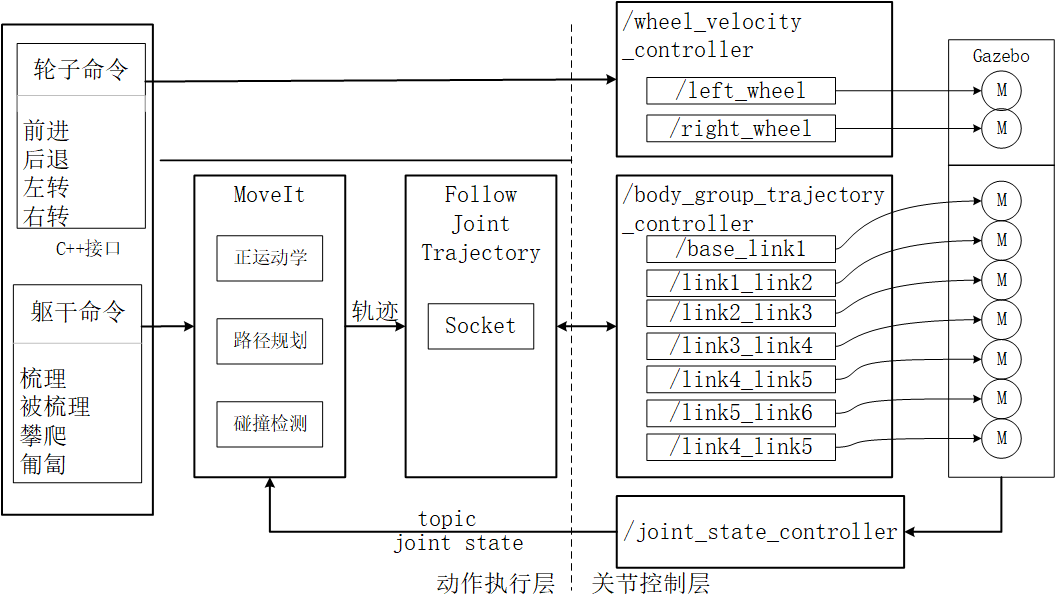
\includegraphics[width=0.6\linewidth]{images/ch03/doactlayer.png}
  \caption{动作执行层数据流图}\label{figure_doactlayer}
\end{figure}
%包括"rat\_rear\_pose"(直立)、"rat\_sniff\_pose"(嗅探)、"rat\_groom\_pose"(梳理)、"rat\_allowgroom\_pose"(被梳理)、"rat\_up\_pose"(攀爬)、"rat\_under\_pose"(匍匐),
\section{行为生成层}
% 仿真环境中作为交互对象和训练目标的机器鼠行为生成机制受到特定规则控制(后称规则鼠),显然其行为模式应当尽可能地模拟生物鼠在实验环境中的表现。虽然利用一成不变的规则指导仿生机器鼠与生物鼠直接交互存在诸多不足,但根据具有统计学意义的生物鼠行为数据库产生机器鼠的行为仍具有较大的可行性。

研究者对生物鼠的行为表现进行了统计并进行了数据分析,结果表明生物鼠不同行为的表现频率不同,并建立了相应的生物鼠行为表现的数据库\cite{ISI:000436213800018}。其研究提供了丰富的关于生物鼠行为表现的统计资料,本文将根据这一研究已揭示的生物鼠不同行为表现概率设计仿真平台行为生成层的行为决策机制。
% \begin{table}[htb]
%   \linespread{1.5}
%   \zihao{5}
%   \centering
%   \caption{生物鼠不同行为的表现概率和次数}\label{table_behavp}
%   \begin{tabular}{p{2cm}<{\centering\arraybackslash}p{6cm}<{\centering\arraybackslash}p{2cm}<{\centering\arraybackslash}}
%     \toprule
%     行为     & 表现概率$p$(以时间计) & 出现次数$m$  \\ \midrule
%     被梳理 & 0.047 & 105 \\
%     接近     & 0.075 & 355 \\
%     跟随     & 0.093 & 259 \\
%     远离     & 0.044 & 387 \\
%     攻击     & 0.01  & 85  \\
%     按压     & 0.006 & 8   \\
%     嗅探     & 0.103 & 506 \\
%     无交互 & 0.586 & 484 \\
%     其他     & 0.036 & 196 \\
%     \bottomrule
%     \end{tabular}
% \end{table}

% 上述研究表明了随机的生物鼠行为中存在着概率上的差异,例如,即便是处于同一实验环境中的两只生物鼠,主要行为模式仍然是无交互($p=0.586$)。依据上述统计数据建立的仿生机器鼠行为产生机制将能够在一定程度上模仿生物鼠的行为。

% 为表现这一概率差异,一个通常做法是利用计算机随机数引擎。为保证精度和良好的随机性,本文利用C++11标准的随机数发生器,将其引擎类定义为shuffle\_order\_engine,将分布类定义为uniform\_int\_distribution,生成范围在$[0,10000)$的随机整数,根据该随机数及表\ref{table_behavp}决定规则鼠的行为表现。

% 同时,生物鼠的行为持续时间往往是不定的\cite{brunswikProbabilityDeterminerRat1939},例如,当生物鼠之间产生亲密的交互行为时,其交互欲望更强烈,相应动作的持续时间往往会比非亲密交互行为的动作更长。为满足这一特性,仿真平台中的机器鼠将以$20~s$为一个周期决定其交互欲望,即当判定当前行为为有效的亲密动作时,交互欲望更强,反之交互欲望将衰退。而有效的亲密动作即为前文所述生物鼠交互的四种常见交互行为(征服、服从、梳理和嗅探)\cite{BarnettSTheRat}。%因此,规则鼠的行为决策机制为图\ref{figure_behavdeci}。
% %\begin{figure}[htb]
% %  \vspace{13pt}
% %  \centering
% %  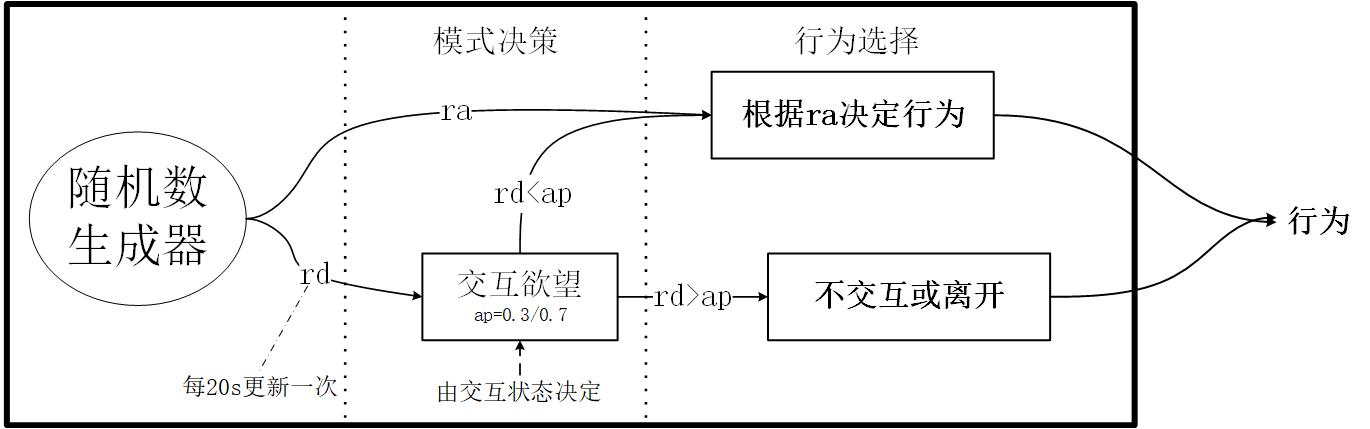
\includegraphics[width=0.95\linewidth]{images/ch03/behavdeci.png}
% %  \caption{规则鼠行为决策机制}\label{figure_behavdeci}
% %\end{figure}

根据不同状态设定不同的动作序列,并从Gazebo仿真环境中获取相应的反馈信息是必要的,相应的仿生机器鼠状态判断机制(图\ref{figure_statecheck})可以通过Gazebo提供的相关话题和服务实现。
\begin{figure}[htb]
  \vspace{3pt}
  \centering
  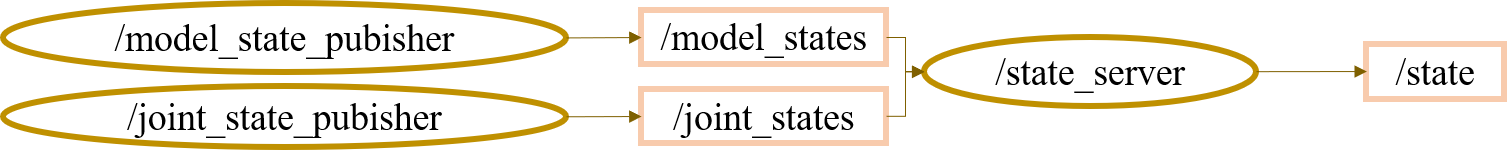
\includegraphics[width=0.95\linewidth]{images/ch03/statecheck.png}
  \caption{仿生机器鼠状态判断机制}\label{figure_statecheck}
\end{figure}

根据上述分析,本文建立的行为生成层数据流为图\ref{figure_behavgene}。
\begin{figure}[htb]
  %\vspace{13pt}
  \centering
  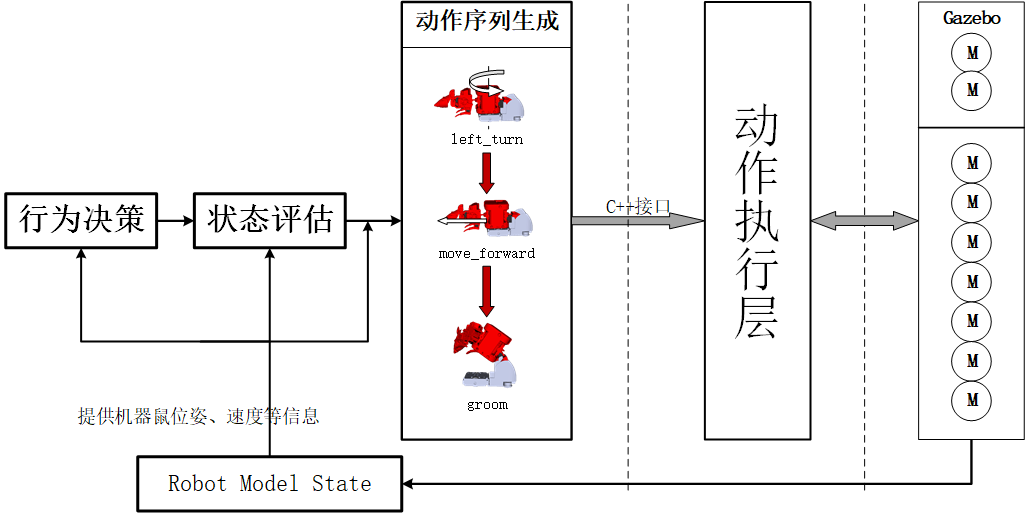
\includegraphics[height=0.25\linewidth]{images/ch03/behavgene.png}
  \caption{行为生成层数据流图(规则鼠)}\label{figure_behavgene}
\end{figure}
